\documentclass{sigchi}

\usepackage{url,graphicx,multirow,color,calc,ulem,threeparttable,tabularx,booktabs,enumitem,subcaption,balance,amsfonts,comment}
\usepackage[group-separator={,}]{siunitx}

% llt: Define a global style for URLs, rather that the default one
\makeatletter
\def\url@leostyle{%
  \@ifundefined{selectfont}{\def\UrlFont{\sf}}{\def\UrlFont{\small\bf\ttfamily}}}
\makeatother
\urlstyle{leo}


% To make various LaTeX processors do the right thing with page size.
\def\pprw{8.5in}
\def\pprh{11in}
\special{papersize=\pprw,\pprh}
\setlength{\paperwidth}{\pprw}
\setlength{\paperheight}{\pprh}
\setlength{\pdfpagewidth}{\pprw}
\setlength{\pdfpageheight}{\pprh}

\usepackage[pdftex]{hyperref}
\hypersetup{
  bookmarksnumbered,
  pdfstartview={FitH},
  colorlinks,
  citecolor=black,
  filecolor=black,
  linkcolor=black,
  urlcolor=black,
  breaklinks=true,
  pdfinfo={
    Title={PocketParker: Pocketsourcing Parking Lot Availability},
    Author={Anandatirtha Nandugudi, Taeyeon Ki, Carl Nuessle and Geoffrey
    Challen},
  }
}

\usepackage[absolute]{textpos}

\setlength{\TPHorizModule}{1in}
\setlength{\TPVertModule}{1in}
\textblockorigin{0.75in}{0.5in}

\usepackage[all]{hypcap}

\input{.xxxnote}
\input{.draft}
\input{.blue}
% 16 Nov 2010 : GWA : Any special macros or other stuff for this particular
%               paper go here.



\begin{document}
\date{}

\numberofauthors{1}

\author{
  \alignauthor Anandatirtha Nandugudi, Taeyeon Ki, Carl Nuessle, and Geoffrey Challen\\
  \affaddr{University at Buffalo}\\
  \email{\{ans25,tki,carlnues,challen\}@buffalo.edu}
}

\title{PocketParker: Pocketsourcing Parking Lot Availability}

\toappear{\fontfamily{ptm}\selectfont Permission to make digital or hard
  copies of all or part of this work for personal or classroom use is granted
  without fee provided that copies are not made or distributed for profit or
  commercial advantage and that copies bear this notice and the full citation
  on the first page. Copyrights for components of this work owned by others
  than the author(s) must be honored. Abstracting with credit is permitted.
  To copy otherwise, or republish, to post on servers or to redistribute to
  lists, requires prior specific permission and/or a fee. Request permissions
  from \href{mailto:permissions@acm.org}{Permissions@acm.org}.\\
  Copyright is held by the owner/author(s). Publication rights licensed to
  ACM.\\
  \href{http://ubicomp.org/ubicomp2014/}{\textit{UbiComp'14}}, September
  13--17, 2014, Seattle, WA, USA\\
  ACM 978-1-4503-2968-2/14/09$\ldots$\$15.00.\\
\href{http://dx.doi.org/10.1145/2632048.2632098}{http://dx.doi.org/10.1145/2632048.2632098}}

\maketitle

\ifdefined\isblue
\begin{textblock}{1}(6.4,0)
\noindent\href{http://blue.cse.buffalo.edu}{
\includegraphics[width=0.6in]{./figures/logos/blue.jpg}}
\end{textblock}
\fi

\begin{abstract}
% <wc:start description="Abstract" max=150>
Searching for parking spots generates frustration and pollution. To address
these parking problems, we present \textit{PocketParker}, a crowdsourcing
system using smartphones to predict parking lot availability. PocketParker is
an example of a subset of crowdsourcing we call \textit{pocketsourcing}.
Pocketsourcing applications require no explicit user input or additional
infrastructure, running effectively without the phone leaving the user's
pocket. PocketParker detects arrivals and departures by leveraging existing
activity recognition algorithms. Detected events are used to maintain per-lot
availability models and respond to queries. By estimating the number of
drivers not using PocketParker, a small fraction of drivers can generate
accurate predictions. Our evaluation shows that PocketParker quickly and
correctly detects parking events and is robust to the presence of hidden
drivers. Camera monitoring of several parking lots as 105~PocketParker users
generated \num{10827}~events over 45~days shows that PocketParker was able to
correctly predict lot availability 94\% of the time.
% <wc:end>

\end{abstract}

\keywords{
  Smartphone sensing; Crowdsourcing; Parking.
}

\category{C.2.4}{Computer-Communication Networks}{Distributed Systems}

\section{Introduction}


Parking lots present a difficult search problem. Drivers lack the visibility
to determine where spots are available, and may spend a non-trivial amount of
time searching for a spot. The problem is difficult enough that WikiHow
includes directions~\cite{wikihow-park} and the Wall Street Journal has
published an online article~\cite{wsj-park} with tips on spot stalking for
shoppers during the holidays. Searching not only generates frustration but
also wastes energy and produces harmful environmental emissions.

Online smartphone application stores such as Google Play and the App Store
teem with apps to locate parking spots. Although some drivers may find these
applications useful, the apps either do not provide real-time parking lot
availability or simply display publicly-available information. Several
research projects have attempted to address these limitations~\cite{4212497,
Chen:2012:COS, Delot:2009:CRP, 5062057, Mathur:2010:PDS} but include
requirements rendering them impractical.  They either require additional
infrastructure~\cite{5062057}, on-vehicle equipment~\cite{Mathur:2010:PDS}
or networking~\cite{Delot:2009:CRP, Mathur:2010:PDS}, or onerous manual user
input~\cite{Chen:2012:COS}. In contrast, we believe the solution is already
in peoples' pockets.

We present \textit{PocketParker}, a system that predicts parking lot
availability using smartphones. Unlike previous approaches, PocketParker
requires no additional infrastructure, no vehicle modifications, and no user
input, only installation on a small percentage of the 100~million smartphones
already in use in the US~\cite{smartphone-numbers}. PocketParker runs
unattended in the background and uses the accelerometer to detect parking lot
arrivals and departures.  These are forwarded to a central server, which
incorporates them into per-lot availability models.  This allows PocketParker
to order lots accurately by the probability that they contain an available
spot.  In general, we consider our approach to be an example of a subset of
crowdsourcing that does not require any manual user input, which we call
\textit{pocketsourcing}.

Predicting parking availability requires the efficient and accurate detection
of parking-related events and the incorporation of the effect of
\textit{hidden drivers}---those not using PocketParker---into our
availability model. We address the first challenge by designing a simple yet
effective event detector which uses the smartphone accelerometer to
efficiently detect arrival and departure events, triggering energy-hungry GPS
acquisition only when necessary. We address the second challenge by designing
an availability estimator that maintains a probability model for each lot
continuously incorporating data from PocketParker clients. We use detected
events both to estimate arrival and departure rates and to make changes in
real time. Part of the key to our approach is the observation that even with
limited information, there are moments when PocketParker can be certain about
the availability of a parking spot in a given lot, and this certainty allows 
PocketParker to assist users.

We perform a careful evaluation of PocketParker using a variety of methods
tailored to each system component. We evaluate our parking event detector in
a controlled environment with eight volunteers participating in ten parking
scenarios. We design a simulator to evaluate our parking availability
estimator, which gives us the flexibility to experiment with a variety of
parameters and parking lot types. Finally, we evaluate the overall
effectiveness of PocketParker by deploying it with 105 smartphones used by
our participants over forty five days. To obtain ground truth, we deploy four
cameras that monitor two parking lots over two weeks. We inspect and
hand-code four days' worth of images of these lots to measure their true
availability. Altogether, our results show the efficiency and accuracy
of PocketParker.

PocketParker has several components
distributed across participating smartphones and a backend server. The rest
of our paper describes each component in detail. We start by presenting
related work in order to distinguish PocketParker from multiple previous
efforts at parking monitoring. In the following two sections we describe two
major components of PocketParker: our parking event detector and availability
model. The evaluation that follows is based both on simulations, controlled
experiments, and a prototype deployment which engaged 105~users.  Finally, we
discuss limitations and future work before concluding the paper.

\begin{comment}
\begin{figure}
\centering
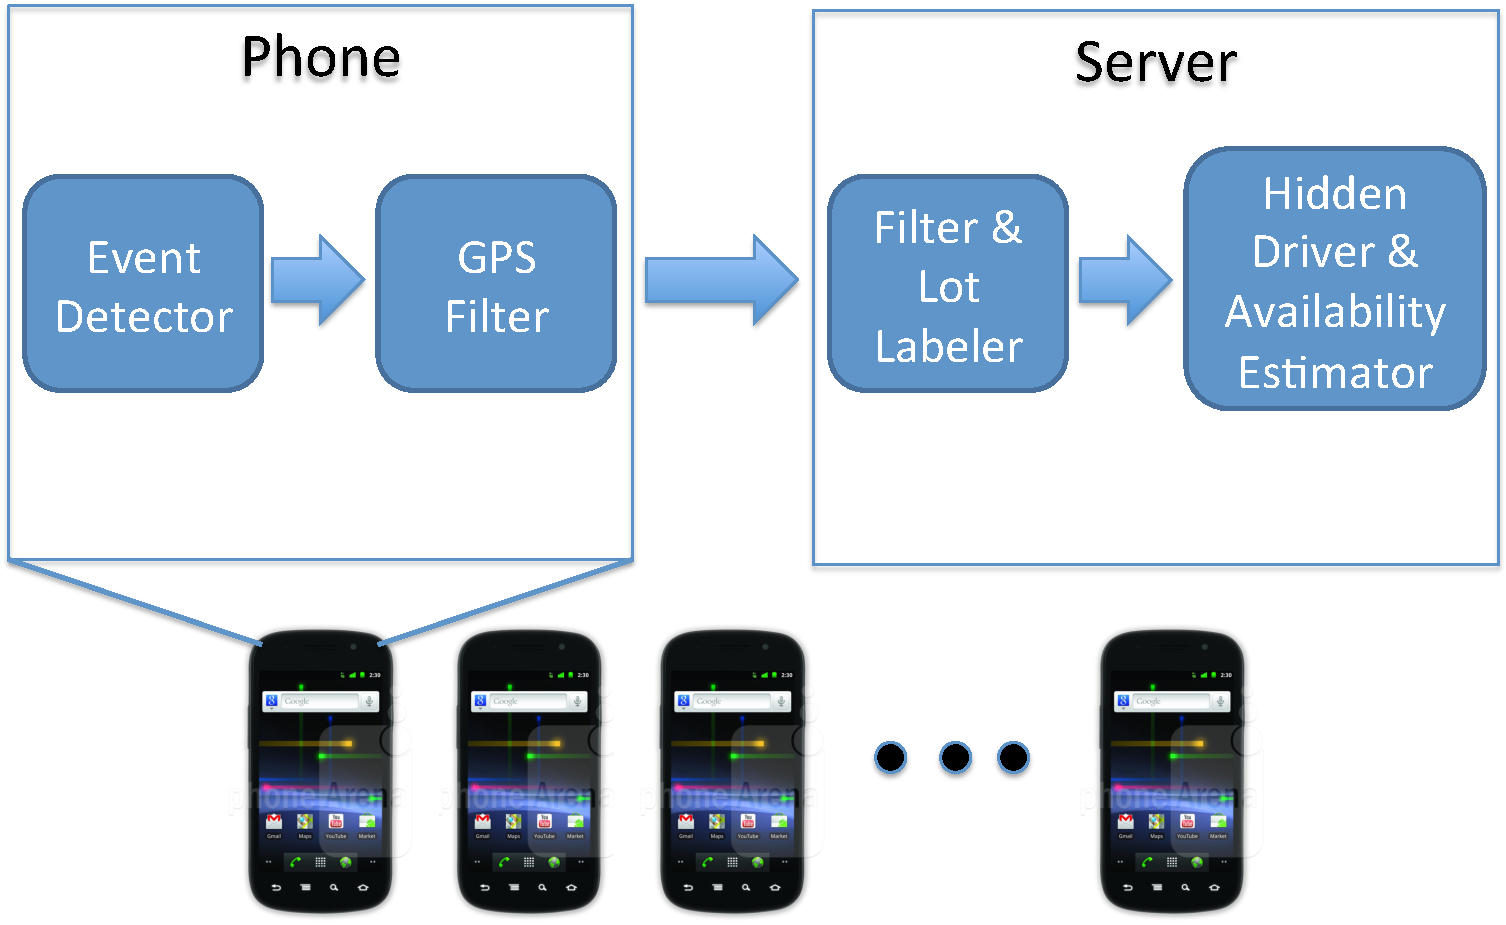
\includegraphics[height=1.5in]{./figures/blockdiagram.pdf}

\caption{\textbf{The PocketParker architecture.} Events generated by an
activity detector running quietly on each smartphone are processed by a
central server and used to estimate parking lot availability.}

\label{fig-arch}
\vspace*{-0.2in}
\end{figure}
\end{comment}

\section{Related Work}
\label{sec-related}

\section{Event Detector}
\label{sec-detector}

\clearpage
\newpage

\section{Availability Estimation}
\label{sec-model}

In order for parking events to be useful, they must be incorporated into a
model allowing us to predict parking lot availability. Our goal is to respond
to queries with the probability that a given parking has a space available,
information that can be used in several ways to determine what lots to search
and in what order. PocketParker's estimator uses the events produced by our
parking event detector both to estimate the rates at which drivers are
searching and departing from the lot and to adjust the availability
probability directly. In this section, we present the design of the
PocketParker parking lot availability estimator and portions of our system
that run on the backend server.

\subsection{Overview}

\begin{figure}
\centering
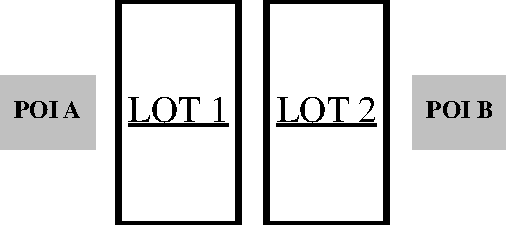
\includegraphics[width=\columnwidth]{./figures/CartoonLot.pdf}

\caption{Example parking lot setup with two lots 1~and~2 and three
destinations A, B and C.}

\label{fig-lots}
\end{figure}

Figure~\ref{fig-lots} shows an example setup with two parking lots and two
destinations used throughout this section. For each lot $l$, PocketParker
maintains a time-varying probability that the lot has $n$ free spots $P_l(t,
X = n)$. While we are mainly interested in the probability that the lot has a
space available $P_l(t, X > 0)$, we maintain separate probabilities for each
number of free spots so that we can manipulate individual probabilities in
response to events and queries as described below. We bound the count
probability distribution to lie between 0 and the capacity of the parking
lot. Section~\ref{subsec-capacity} briefly describes how PocketParker
estimates lot capacity.

PocketParker's estimator receives two types of events: arrivals and
departures. However, for each arrival in a given lot, a number of additional
lots may have been searched unsuccessfully, information critical to the
accuracy of our availability model. Section~\ref{subsec-lots} describes how
PocketParker determines relationships between parking lots, and
Section~\ref{subsec-implicit} describes how we combine that information with
arrivals to estimate implicit search behavior.

Between events we want to maintain our availability model by estimating the
rate at which departures and searches are taking place. PocketParker must use
the events it can detect to estimate the rate at which events are taking
place in the lot, which includes the effect of drivers not using
PocketParker, which we call \textit{hidden drivers}. Accomplishing this
requires that we estimate the ratio between monitored and hidden drivers, and
we describe an approach to doing so in Section~\ref{subsec-hidden}. With an
estimate of the hidden driver ratio, we can scale the search and departure
rates according, described in Section~\ref{subsec-rates}. Finally,
Section~\ref{subsec-online} describes how we integrate all of this
information to update our availability estimate as arrival and departure
events are received.

\subsection{Estimating Lot Capacity}
\label{subsec-capacity}

PocketParker requires an estimate of lot capacity $C$ in several places.
First, we use this estimate to bound $P_l(t)$ such that $P_l(t, X > C) =
0\;\forall\;t$. Second, we use the capacity to determine the number of hidden
drivers, explained in more detail in Section~\ref{subsec-hidden}.

Recall from Section~\ref{FIXME} that our false-positive filter uses knowledge
of the location of lots obtained from the OpenStreetMap database. We estimate
the capacity of each lot by converting the location of the lot into a size
and dividing by the size of an average parking spot. We use the parking lot design
standards provided in \cite{parkingdesign} to estimate the number of spots after estimating the 
area of the parking lot from which we detect an park event. \ref{} Shows our estimation accuracy 
for five lots in our campus.XXXnote \XXXnote{Anand and
Taeyeon, add capacity estimation stuff here. What is the size of the spot
that we determined? Reference for that. Estimates for each of the lots we
used and comparison with the true counts.} Errors in the capacity can result
if the size of parking spots in the lot differ from our estimate, or if the
parking lot is not efficiently packet with spots. Given the incentive of
parking lot designers to maximize capacity, we believe that the second case
will be unlikely. Parking spot sizes, however, may vary significantly from
lot to lot or based on the lot's location. To improve our estimate, we may
need to incorporate location-specific parking spot size estimates.
Alternatively, mapping databases may be directly annotated with the number of
spots per lot.

\subsection{Lot Relationships}
\label{subsec-lots}

PocketParker's detector identifies only arrivals and departures. However,
understanding and incorporating search behavior is critical to our model. For
example, if we observe the arrival rate fall at a given lot, it may be
because the lot is full, or it may be simply because fewer drivers are
arriving and the lot still has many spaces available.

In order to estimate search behavior, we need to understand the relationships
between parking lots. This requires two additional pieces of data about each
lot: one or multiple destinations, and a desirability index. The destination
represents the place the user is going when they park in a given lot, and
note that some lots may be associated with multiple destinations. In
Figure~\ref{fig-lots}, lot~1 may be associated with destinations A, B and C;
while lot~2 is only linked to B.

The desirability index produces an ordering of lots associated with a given
point-of-interest based on how preferable they are compared with other lots.
We assume that most users will park in desirable lots if they are available,
and may have searched in more desirable lots before parking in a lot
desirable lot. In Figure~\ref{fig-lots}, if Lot~2 is associated with
destination~A it will probably receive a lower desirability score than Lot~1
because it is further away.

While this information is not currently part of open mapping databases, we
believe that it is straightforward to collect. Parking lot operators and
business owners can annotate the mapping database with destinations for each
lot. In addition, data from navigation tools may be able to automatically
link destinations with lots by noting where users park after requesting
directions to a particular place. The desirability index may also be
determined by navigation tools observing what lots are searched by users on
their way to a particular destination. Lacking these traces, simple proximity
to the destination may determine the desirability index directly. As example
of this automatic annotation, in Figure~\ref{fig-lots} if both lot~1~and~2 are
associated with destination~A, we can consider lot~2 less desirable than
lot~1 because lot~1 lies between it and the destination.

\subsection{Implicit Searches}
\label{subsec-implicit}

With an understanding of lot relationships we can use observed arrivals to
model implicit---or unobserved---searches. When a user parks in a given lot,
we use the desirability index of the lot to add unsuccessful searches in more
desirable lots associated with the some destination. There are two challenges
to this approach. First, as described above, lots may be associated with
multiple destinations. Second, the user may not have actually performed the
search. After discussing both of these issues below,
Section~\ref{subsec-online} describe below how PocketParker incorporates the
information from implicit searches in a way sensitive to these uncertainties.

\subsubsection{Determining the destination}

If a lot is associated with multiple destinations, we cannot uniquely
determine the destination of the user. However, this only becomes important
if the two destinations would produce different desirability rankings for
affected lots. For example, in Figure~\ref{fig-lots}, if lots 1~and~2 are
both associated with destinations A~and~C, but not with B, then an arrival
with an unknown destination into lot~2 can always be used to generate an
implicit search in lot~1, since the desirability ranking for the two lots are
unchanged if the destination is either A~or~C. However, if both lots~1~and~2
are associated with all three destinations, then an arrival detected in lot~2
becomes more ambiguous. If the user was trying to go to destination~A, it may
mean that lot~1 was searched and is full; however, if they were trying to go
to destination~B, it may not indicate anything about lot~1. 

If lot destination annotations are generated by mapping software, we can use
this data to estimate the probability that a user is going to each of the
destinations associated with a particular lot. Instead of generating a single
implicit search in one lot, we generate multiple implicit searches in each of
the lots weighted by the destination probabilities. Lacking this arrival
data, we simply generate implicit searches in each destination associated
with a given lot.

\subsubsection{Speculative searches}

If we do not directly observe a user searching a lot before we detect an
arrival, we cannot be certain that they performed the search. If the
unsearched but preferable lot was available, they may not have searched it
because they prefer to choose the first available spot, enjoy the exercise of
walking farther to their destination, or want to irritate their passengers.
However, these are not the type of users we believe would benefit from or use
our PocketParker application, since finding a non-optimal parking spot is
fairly simple in most cases.

A more interesting case is where a user has not performed a search before
parking in a less-desirable lot because they \textit{believe} the more
desirable lot to be full. Users that park regularly at the same destination
usually have their own mental models for the availability of spots in certain
lots, causing them to discard those lots without searching them if they
believe the probability of finding a spot in the desirable lot is low. While
this behavior can cause users to miss available spots, these speculative
searches are useful inputs into our PocketParker model since it represents
what lots users think are full.

A final corner case that PocketParker does not handle is if all of the lots
for a given destination are full, and many undetected unsuccessful searches
are taking place. On one hand, if all lots are full then the availability of
spots is determined by departures, not arrivals, and so search data is
useless anyway. On the other hand, we would still like to identify this
situation for users that would prefer to avoid destinations where it is
difficult to park. While discussing future work in Section~\ref{sec-future},
we point out how integrating PocketParker into existing navigation
applications could address this problem by making searches explicit, rather
than implicit.

\subsection{Hidden Driver Estimation}
\label{subsec-hidden}

Monitored PocketParker users compete for parking spaces with unmonitored
users, which we call \textit{hidden drivers}. While we assume that
PocketParker users are generally representative of the entire driving
population, we do not assume that all or even a large fraction of drivers
will download and install PocketParker and we want our system to still
provide accurate predictions with the limited information caused by hidden
drivers. To accomplish this, PocketParker needs to estimate percentage of
drivers that are monitored, which we call the \textit{monitored fraction}. A
low monitored fraction indicates that few users are using PocketParker,
whereas a high monitored fraction means that we are receiving inputs from
most drivers. Put another way, the amount of uncertainty PocketParker must
face when predicting lot availability is inversely-proportional to the
monitored fraction.

\subsubsection{Importance of monitored fraction estimation}

Two examples will illustrate why we need this information and how it is used.
First, when a monitored driver leaves a parking lot, the monitored fraction
determines how long PocketParker will predict that a spot in that lot is
available. As the monitored fraction increases, the probability of
PocketParker seeing the arrival into the lot that occupies that spot
increases, and we can increase the amount of time that we estimate a spot is
available. On the other hand, as the monitored fraction decreases we see
fewer arrivals and are faced with more uncertainty. Hence, PocketParker
reduces the amount of time it predicts the spot is available. In
Section~\ref{subsec-online} we describe how hidden drivers influence the
changes to the availability model made when arrivals and departures are
detected.

Second, PocketParker uses the arrival and departure rates of monitored
drivers to estimate changes to parking lot availability over time. Here we
must scale the observed number of events to the actual number of events,
which requires an estimate of the monitored fraction.
Section~\ref{subsec-rates} describes how the monitored rate is used as an
input into rate estimation and scaling.

\subsubsection{Estimating the monitored fraction}

\begin{figure}
\centering
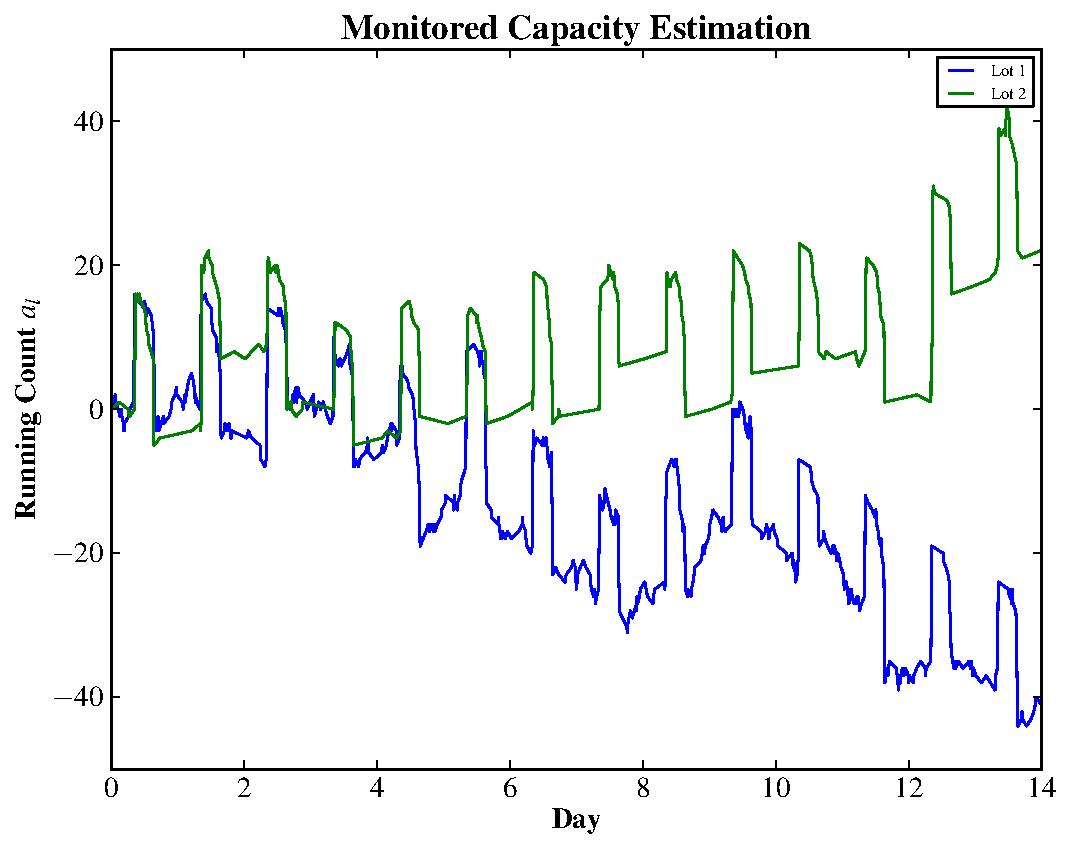
\includegraphics[width=\columnwidth]{./simulator/figures/capacity.pdf}

\caption{Example of capacity estimation for two parking lots using a running
count.}

\label{fig-capacityexample}
\end{figure}

PocketParker estimates the monitored fraction by first determining the
monitored capacity---the capacity of the lot measured by monitored
drivers---and then using our estimate of the lot capacity discussed in
Section~\ref{subsec-capacity}. Specifically, given a lot with capacity $C$,
the monitored fraction can be estimated as $f_m = \frac{C_m}{C}$. Our task
then becomes estimating the monitored capacity $C_m$.

To estimate the monitored capacity we maintain a running count $a_l$ for each
lot. When a monitored driver arrives in the lot, we decrement $a_l$; when a
monitored driver leaves the lot, we increment $a_l$. We can consider $a_l$ as
a estimate of the number of spots available in the lot scaled by $f_m$,
although we do not bound $a_l$ to be below the lot capacity or greater than
zero.

Figure~\ref{fig-capacityexample} shows an example of the running count for
two related lots over seven days using data generated by our lot simulator
described in Section~\ref{FIXME}. Both lots have capacity 200 and the actual
monitored fraction is 0.1. As the data shows, the running count experiences
long-period (greater than one day) fluctuations due to events missed by our
event detector and the randomness associated with the small percentage of
drivers being monitored. However, the data also contains short-period (less
than one day) fluctuations caused by the dynamics of the lot being monitored,
and these fluctuations are roughly the size of the monitored capacity $C_m$,
which in this case is 20 spots.

This observation motivates the design of our monitored capacity estimator.
First, we remove the long-period fluctuations from $a_l$ by applying a moving
average filter with a window length of 24~hours.
Figure~\ref{fig-capacityexample} shows the filtered data. Next, we identify
the largest availability swing over each 24~hour window. Finally, we average
multiple swings together for a period of days to determine the final
estimate. We expect this approach to work well on lots that fill on a regular
basis. For lots that do not fill, or do not fill regularly, we may need to
produce a weighted sum where larger swings are weighted more heavily given
our assumption that they more accurately measure the true monitored capacity
of the lot.

\subsection{Rate Estimation}
\label{subsec-rates}

\subsection{Online Updates}
\label{subsec-online}

Each arrival and departure received represent strong positive information:
moments when PocketParker knows either that a spot just existed (arrival) or
now exists (departure). Unsuccessful searches, in contrast, represent weaker
negative information, either because they may not have actually been observed
by PocketParker (unannotated) or so may not have actually taken place, or
because they may not have been thorough (annotated).

\begin{figure*}[t]
\centering
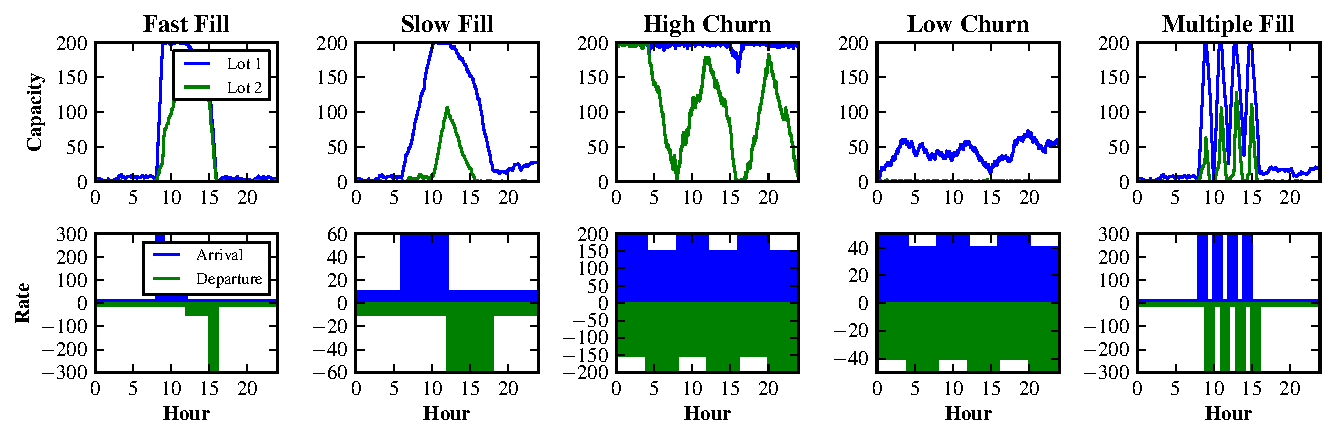
\includegraphics[width=\textwidth]{./simulator/figures/lots.pdf}

\caption{\textbf{Description of each type of lot simulated.} Five different
lots with different behaviors were used.}

\label{fig-lotsdescription}
\end{figure*}

\newpage
\section{Evaluation}
\label{sec-evaluation}

We evaluated PocketParker in three ways. First, we conducted a controlled
experiment to determine the best parameter settings for our event detector.
Second, we implemented a parking lot simulator to experiment with various
kinds of lots under differing monitored fractions. Finally, we performed a
large-scale deployment of PocketParker on our campus and used it to monitor
two lots, with camera monitoring used to ground truth our predictions. Our
evaluations confirm that PocketParker is efficient and accurate.

\subsection{Detector Experiment}

\begin{figure}[t]
\centering
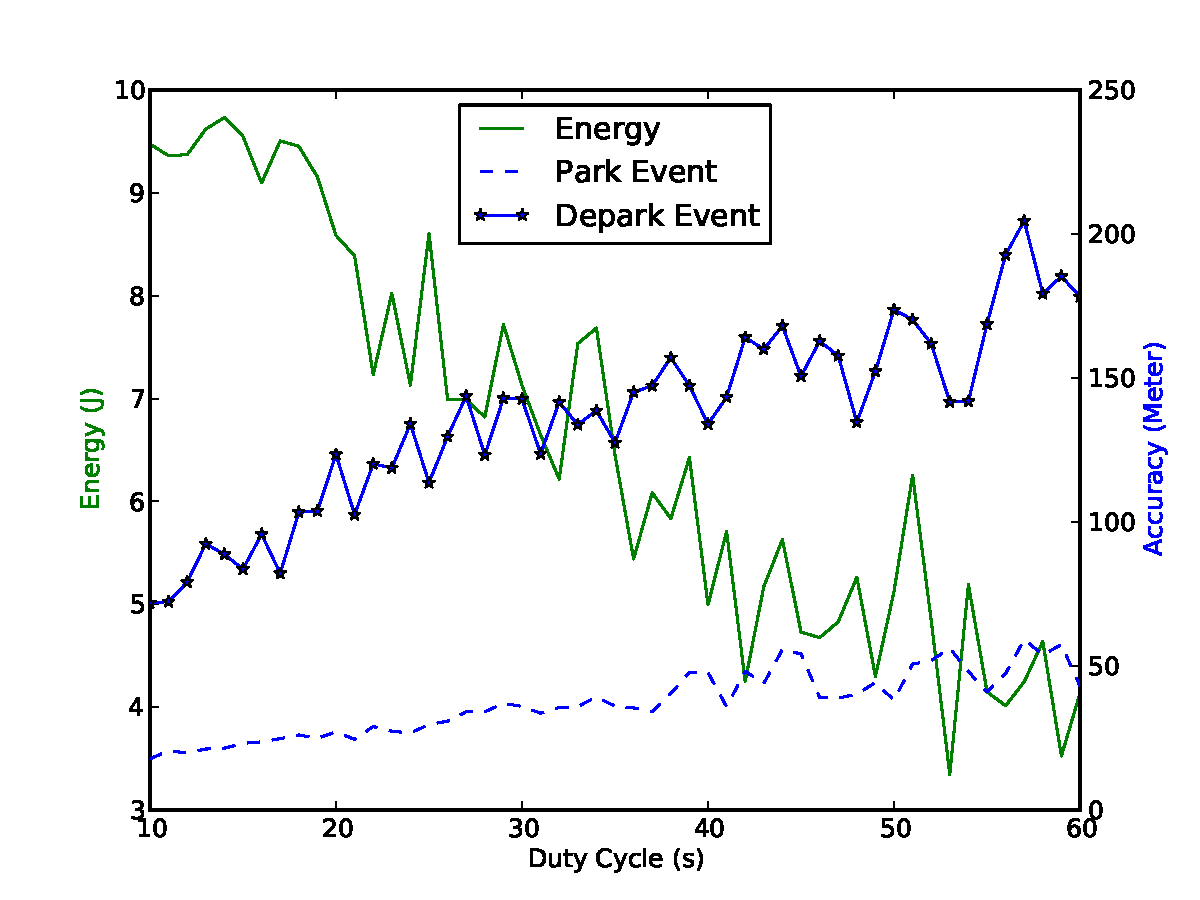
\includegraphics[width=\columnwidth]{./figures/Energy_accuracy.pdf}

\caption{\textbf{Power usage vs. detector accuracy.} Energy usage by
PocketParker is low at all duty cycles, so we chose a high duty cycle to
improve accuracy.}

\label{fig-energy}
\end{figure}

\newcolumntype{b}{>{\hsize=1.4\hsize}X}
\newcolumntype{s}{>{\hsize=.6\hsize}X}
\begin{table}[t]
{\small
\begin{threeparttable}
\begin{tabularx}{\columnwidth}{b s b s}
  {{\textbf{Carry Location}}} & {{\textbf{Count}}} &
  {{\textbf{Car Location}}} &
  {{\textbf{Count}}} \\
 \hline
In hand & 18 & Cup holder & 16 \\
Side bag & 10 & Car seat  & 9 \\
Back pack & 10 & Side bag & 10 \\
In hand talking & 7 & Back pack & 9 \\
Front pocket & 14 & Front pocket & 14 \\
Jacket pocket & 14 & Jacket pocket & 14 \\
Back pocket & 7 & Back pocket & 14 \\
\end{tabularx}
\end{threeparttable}
\caption{\textbf{Carry and car location for detector experiment.}
Eight participants generated 80 runs, carrying and placing the
phone in their car in many ways.}
\label{table-experiment}
}
\vspace*{-0.1in}
\end{table}


To determine the right parameter settings for our transition detector, we
conducted a controlled experiment. During this experiment, accelerometer and
GPS data was collected and stored continuously on each device, and
participants were asked to manually label each transition into and out of the
car. Afterwards, data was processed by a Python simulator implementing the
identical algorithm used by the PocketParker application, allowing us measure
accuracy and energy consumption as a function of the detector duty cycle.

Eight volunteers participated, including seven men and one woman. Seven were
right-handed and one was left-handed. Each was asked to conduct the same
experiment ten times: (1) carrying the instrumented phone, walk to their car;
(2) label departure; (3) drive around campus briefly; (4) park and label
arrival; (5) return inside. Since the way the phone is carried while walking
and placed in the car while driving affects the accelerometer readings, care
was taken to generate a good mix of carry and car location styles.
Table~\ref{table-experiment} shows the breakdown. The experiment permitted us
to obtain sensing data from a cross section of individuals possessing
different body morphologies, habits of driving cars, and ways of handling
mobile devices.

Figure~\ref{fig-energy} displays the tradeoff between energy usage and
detection accuracy as a function of the PocketParker duty cycle. Here we
combine an active period of 5s with a inactive period of variable length,
between 5~and~55s, for an overall duty cycle between 0.5 and 0.06. Our
simulator uses energy numbers from the Android Fuel Gauge application
to estimate average power consumption.  This graph measures the accuracy of
detected events in terms of distance from the actual location of the event
labeled by the participant.

As expected, longer duty cycles consume less energy but produce longer
detection latencies which translate into higher distances from the event
location. Note also that departures have higher location error than arrivals
because departing users are driving and therefore traveling more rapidly.
Overall power usage by PocketParker is low, under 10~mW at all duty cycles.
Because PocketParker's ability to map parking events into lots is affected by
the detection distance accuracy, we chose a low total period of 15~s for a
0.25 duty cycle. This allows PocketParker to determine location to within
25~m for arrivals and 80~m for departures. Power consumption at this duty
cycle is 8~mW, representing 4.2\% of the capacity of a 1500~mAh battery over
24~hours.

\begin{figure}
\centering
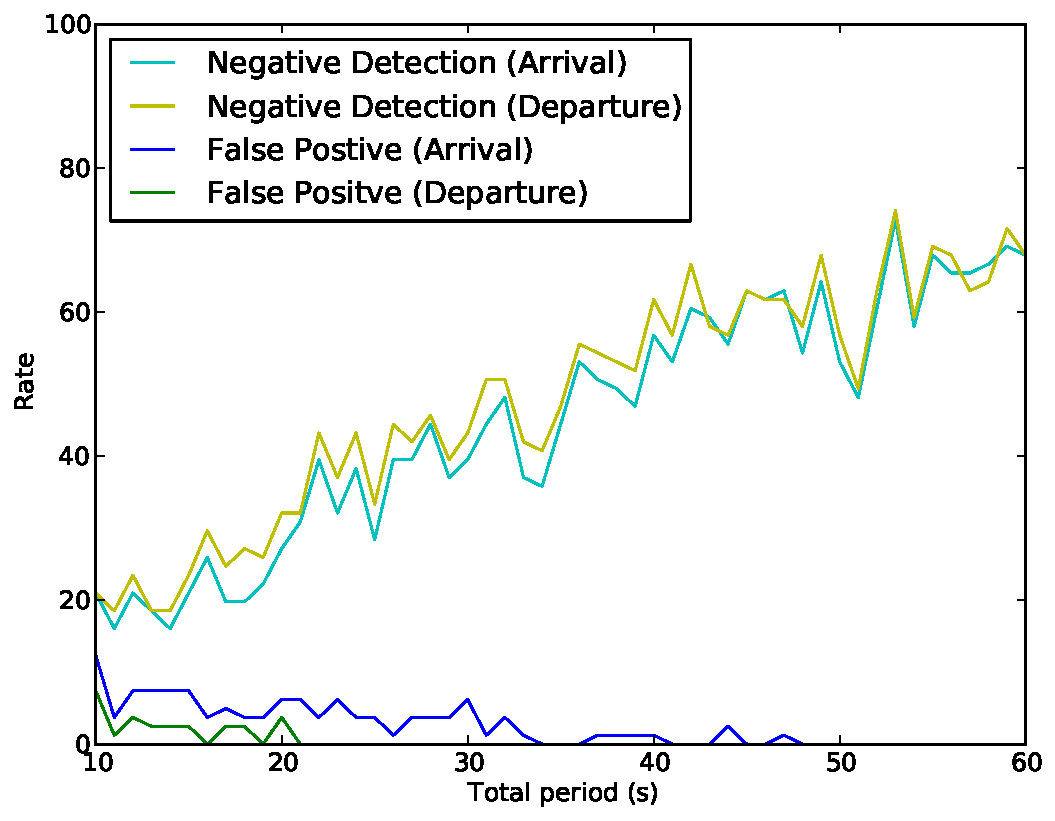
\includegraphics[width=\columnwidth]{./figures/Rate_FP_and_ND.pdf}

\caption{\textbf{False positive and negative rates as a function of detector
duty cycle.}} 

\label{fig-falsepositives}
\end{figure}

Using the same data we also examine the false positive and negative rates for
arrivals and departures. This is important since, without explicit user
input, it would be impossible to determine this information while
PocketParker is in use. Figure~\ref{fig-falsepositives} shows PocketParker
can detect 80\% of arrival and departure events correctly at the 0.25 duty
cycle we use. False positive rates are already quite low, and this is before
we apply our GPS availability filter and lot location filters. False
positives decline as the duty cycle decreases because PocketParker has fewer
opportunities to detect user activity.
\begin{comment}
\begin{figure}[t]
\centering
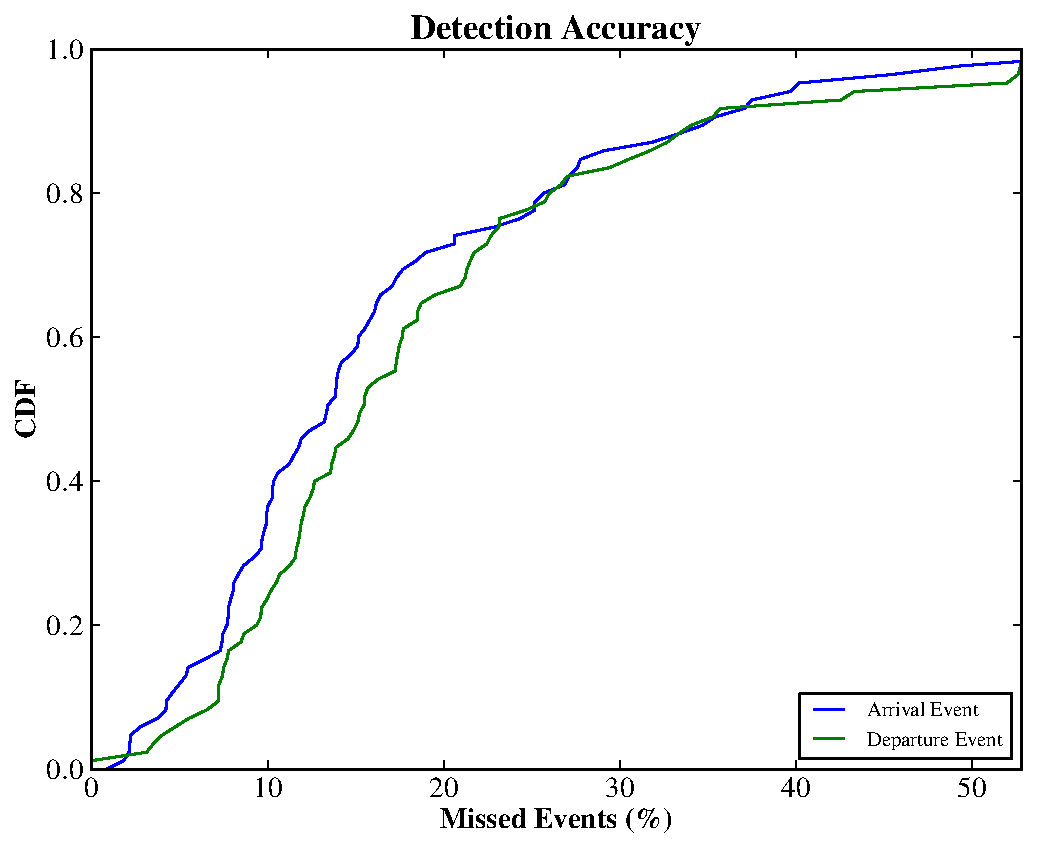
\includegraphics[width=\columnwidth]{./figures/MissedEvents_CDF.pdf}

\caption{\textbf{The percentage of missed parking Events.}}

\label{fig-missedevents}
\end{figure}

Figure~\ref{fig-missedevents} shows that PocketParker detects parking events 
faithfully: 80\% of users missed less than 25\% parking events. The main reason 
is because PocketParker has transition time threshold of 5 minutes. Therefore, 
PocketParker requires a minimum of 5 minutes to detect an user transition event
(from walking to driving or driving to walking). 
\end{comment}

\subsection{Simulation Results}
\label{subsec-simulator}

To experiment with PocketParker in a more controlled setting, we implemented
a parking lot simulator in Python. Our simulator allows us to simulate any
number of parking lots associated with any number of points of interest with
varying desirability levels. For simplicity during our evaluation, we
simulate two lots 1~and~2 with lot~1 filling before lot~2, although lot
choice by simulated drivers is randomly weighted. Particularly for evaluating
our monitored fraction estimation, we use five types of lots that fill and
empty differently:

\begin{itemize}

\item \textbf{Fast Fill} and \textbf{Slow Fill} fill once per day quickly or
slowly, like a lot associated with a place of work.

\item \textbf{Multiple Fill} represents a lot that rapidly fills and empties
repeatedly during each day, like a campus lot or movie theater.

\item \textbf{High Churn} starts with lot~1 full and experiences continuously
high arrival and departures rates, like an airport parking lot.

\item \textbf{Low Churn} represents underutilized lots that never completely
fill, with lot~2 almost completely unused.

\end{itemize}

Figure~\ref{fig-lotsdescription} shows the arrival and departure rates for
each of the types of lot as well as the resulting per-lot capacity.

\begin{figure*}
\centering
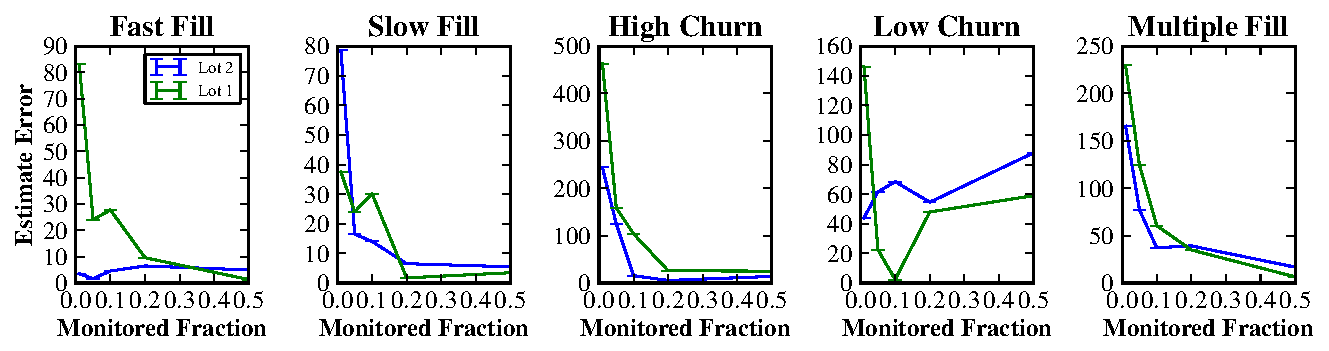
\includegraphics[width=\textwidth]{./simulator/figures/capacity_experiment.pdf}

\caption{\textbf{Errors in monitored fraction estimation.} Currently
PocketParker is better at estimating the monitored fraction when lots fill
and empty regularly.}

\label{fig-capacityerrors}
\end{figure*}

\subsubsection{Monitored fraction estimation}

Earlier we described our approach to estimated the monitored fraction, a
parameter important to the operation of the PocketParker availability
estimator. Figure~\ref{fig-capacityerrors} shows the results of 10 random
simulations for each lot type. In each case, the monitored fraction estimator
uses a weeks worth of data and proceeds as described previously. The error in
the monitored fraction estimate is shown as a function of the actual
monitored fraction for the simulation used.

For the five types of lots, we would expect PocketParker to do better
monitored fraction estimation when lots fill regularly---Fast Fill, Slow
Fill, and Multiple Fill---and poorly when they do fill erratically or not at
all---High and Low Churn. The results in Figure~\ref{fig-capacityerrors}
generally follow this pattern. Errors for High Churn are quite high, and Low
Churn errors persist even at high monitored driver fractions. This is
natural, as the Low Churn lot never fills.  By contrast, the accuracy rate for
the Fast, Slow and Multiple Fill models improve with an increasing fraction of
monitored drivers.

\begin{figure}[t]
\centering
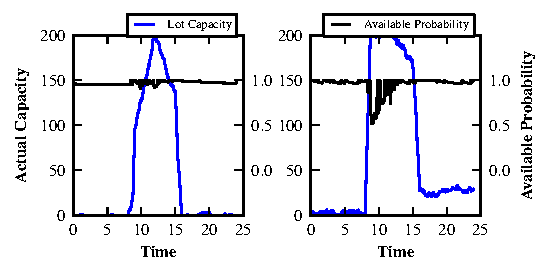
\includegraphics[width=3.325in]{./simulator/figures/tracking_fastfill_horizontal.pdf}

\caption{\textbf{Availability probabilities tracking lot capacity.} Dips in
the availability probability correspond to times when PocketParker believes
the lot is full. Discontinuities are caused by departures, which set the
instantaneous probability that the lot is available to 1.0.}

\label{fig-trackingexample}
\end{figure}

\subsubsection{Probability and availability}

We now consider how PocketParker adjusts lot availability probabilities.  It
uses these probabilities to rank available lots in response to queries.
Figure~\ref{fig-trackingexample} shows a 24~hour simulation of a Fast Fill
parking lot with a monitored fraction of 0.1 and a 10\% error in the
estimation of the monitored fraction. The ground truth capacity of the lot as
simulated is plotted next to the PocketParker probability that the lot has an
available spot. At the beginning, both lots are marked as free. After lot~1
fills and lot~2 begins to fill, which generates implicit searches
in lot~1, the availability probability of lot~1 drops. It spikes upward
repeatedly due to departures from lot~1---which reset the short-term
probability of an available spot back to 1---but does not equal the
probability for lot~2 again until the point when the departure rate for lot~1
climbs.

\subsubsection{Prediction accuracy}

\begin{table}[t]
\begin{threeparttable}
{\small
\begin{tabularx}{\columnwidth}{Xrrrrr}
\multicolumn{1}{c}{\textbf{Type}} & 
\multicolumn{1}{c}{\textbf{$f_m$}} & 
\multicolumn{1}{c}{\textbf{$f_m$ Error}} & 
\multicolumn{1}{c}{\textbf{Correct}} & 
\multicolumn{1}{c}{\textbf{Missed}} & 
\multicolumn{1}{c}{\textbf{Waste}}\\ \toprule

\textbf{Campus} & & & & & \\
\midrule
& 0.20 & 0.10 & 100.0 \% & 0.0 \% & 0.0 \% \\
\textbf{Fast Fill} & & & & & \\
\midrule
& 0.01 & 0.10 & 75.1 \% & 24.7 \% & 0.2 \% \\
& 0.05 & 0.10 & 72.3 \% & 26.2 \% & 1.5 \% \\
& 0.10 & 0.10 & 80.0 \% & 15.6 \% & 4.4 \% \\
& 0.10 & 0.20 & 86.6 \% & 11.2 \% & 2.2 \% \\
& 0.10 & 0.50 & 89.7 \% & 7.7 \% & 2.7 \% \\
& 0.10 & 1.00 & 93.0 \% & 4.8 \% & 2.2 \% \\
& 0.20 & 0.10 & 87.9 \% & 8.5 \% & 3.6 \% \\
& 0.50 & 0.10 & 94.0 \% & 5.0 \% & 1.0 \% \\
\textbf{High Churn} & & & & & \\
\midrule
& 0.01 & 0.10 & 54.0 \% & 0.0 \% & 46.0 \% \\
& 0.05 & 0.10 & 55.3 \% & 0.0 \% & 44.7 \% \\
& 0.10 & 0.10 & 63.6 \% & 0.0 \% & 36.4 \% \\
& 0.10 & 0.20 & 62.2 \% & 0.0 \% & 37.8 \% \\
& 0.10 & 0.50 & 60.1 \% & 0.0 \% & 39.9 \% \\
& 0.10 & 1.00 & 61.8 \% & 0.0 \% & 38.2 \% \\
& 0.20 & 0.10 & 64.0 \% & 0.0 \% & 36.0 \% \\
& 0.50 & 0.10 & 70.6 \% & 0.0 \% & 29.4 \% \\
\textbf{Low Churn} & & & & & \\
\midrule
& 0.01 & 0.10 & 98.4 \% & 0.0 \% & 1.6 \% \\
& 0.05 & 0.10 & 89.1 \% & 0.0 \% & 10.9 \% \\
& 0.10 & 0.10 & 94.1 \% & 0.0 \% & 5.9 \% \\
& 0.10 & 0.20 & 91.0 \% & 0.0 \% & 9.0 \% \\
& 0.10 & 0.50 & 87.9 \% & 0.0 \% & 12.1 \% \\
& 0.10 & 1.00 & 87.8 \% & 0.0 \% & 12.2 \% \\
& 0.20 & 0.10 & 92.5 \% & 0.0 \% & 7.5 \% \\
& 0.50 & 0.10 & 91.6 \% & 0.0 \% & 8.4 \% \\
\textbf{Multiple Fill} & & & & & \\
\midrule
& 0.01 & 0.10 & 51.4 \% & 42.8 \% & 5.8 \% \\
& 0.05 & 0.10 & 71.2 \% & 26.0 \% & 2.9 \% \\
& 0.10 & 0.10 & 85.2 \% & 13.2 \% & 1.6 \% \\
& 0.10 & 0.20 & 79.4 \% & 17.5 \% & 3.1 \% \\
& 0.10 & 0.50 & 86.2 \% & 12.7 \% & 1.1 \% \\
& 0.10 & 1.00 & 77.6 \% & 20.9 \% & 1.5 \% \\
& 0.20 & 0.10 & 92.1 \% & 7.5 \% & 0.5 \% \\
& 0.50 & 0.10 & 91.6 \% & 7.8 \% & 0.6 \% \\
\textbf{Slow Fill} & & & & & \\
\midrule
& 0.01 & 0.10 & 70.7 \% & 26.0 \% & 3.2 \% \\
& 0.05 & 0.10 & 78.8 \% & 17.5 \% & 3.7 \% \\
& 0.10 & 0.10 & 82.1 \% & 13.3 \% & 4.6 \% \\
& 0.10 & 0.20 & 75.4 \% & 15.2 \% & 9.4 \% \\
& 0.10 & 0.50 & 80.5 \% & 19.3 \% & 0.2 \% \\
& 0.10 & 1.00 & 85.2 \% & 12.5 \% & 2.3 \% \\
& 0.20 & 0.10 & 87.8 \% & 9.8 \% & 2.4 \% \\
& 0.50 & 0.10 & 93.8 \% & 5.6 \% & 0.6 \% \\
\end{tabularx}
}
\caption{\textbf{Accuracy of PocketParker predictions for various kinds of lots and parameters.}}
\label{table-accuracy}
\end{threeparttable}
\end{table}



PocketParker exists to help drivers park efficiently.  To examine its
prediction accuracy, we have PocketParker rank two model lots in order of
preference at regular timesteps and then compare these results with the ground
truth from a simulator.  Finally, we categorize the results as a correct
prediction, a missed opportunity---a case where a more desirable lot was
available than the one that PocketParker recommended---or a waste of
time---where PocketParker sent the user to a full lot.
Table~\ref{table-accuracy} shows data results from simulations run using
varying monitored fractions$f_m$ of drivers.

\begin{figure}[t]
\centering
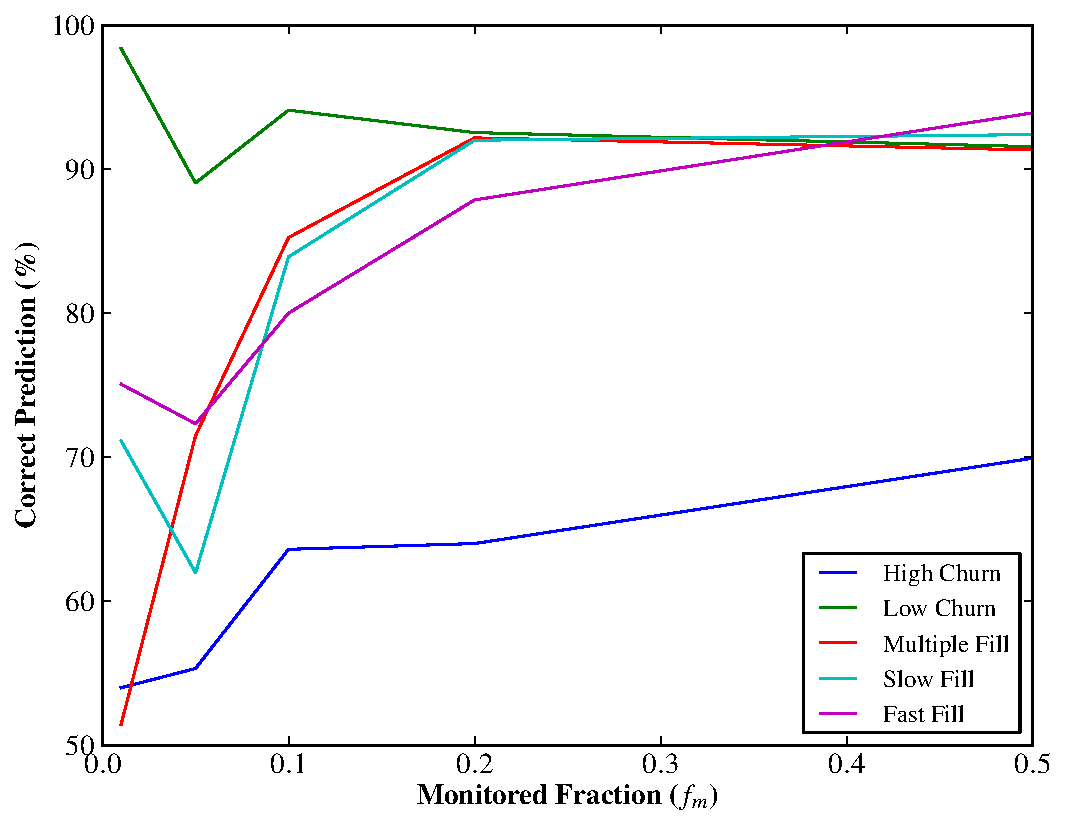
\includegraphics[width=\columnwidth]{./simulator/figures/accuracy_graph.pdf}

\caption{\textbf{Accuracy predictions for various kind of lots and parameters.}}
\label{fig-accuracy}
\vspace*{-0.25in}
\end{figure}

Also, Figure~\ref{fig-accuracy} shows that several trends can be observed 
in the results. First, overall PocketParker does well on most lot types. 
The High Churn lot presents the greatest difficulty, which we would expect 
since its large number of incoming and outgoing drivers make prediction 
difficult. We are also concerned that the High Churn errors are largely 
waste of time errors, indicating that PocketParker is frequently sending 
drivers to the wrong lot.  This is likely because it is predicting that 
spots are available longer than they actually are. Clearly more work is 
needed to determine the right approach for High Churn lots.

Excluding the High Churn lot, the lot with the lowest correct percentage with
a $f_m > 0.1$ is 80\% for the Slow Fill lot.  Accuracy for all lots above
this $f_m$ is consistently good for all lots save the High Churn model.  The
Low Churn lot does have a small number of errors but this is because both lots
are usually empty.

An unavoidable lower bound to accuracy is imposed by the frequency of parking
PocketParker has the most information about lot availability during periods
of parking events. Once such information stops, prediction uncertainty
grows.  Thus, to the degree that PocketParker queries follow a pattern of
arrivals and departures, it will have fresh data and do well.

\subsection{Deployment}

\begin{figure}
\centering
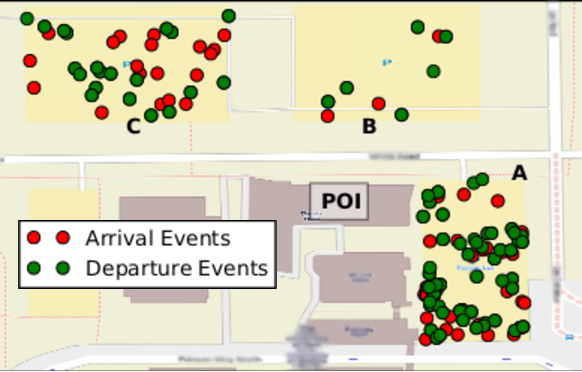
\includegraphics[trim=0 0 0 1mm,clip, width=\columnwidth]{./figures/smallEventsOnThreeParkingLot-anon.pdf}

\caption{\textbf{Map showing 217~parking events detected by PocketParker
during our forty-five-day deployment in three key lots.}  These were
generated by 26 participants.  Lot~A is considered the most desirable of the
three lots, a fact reflected in the higher event density of this lot.  
Lots~A~and~B were monitored by cameras to establish ground truth}

\label{fig-events}
\end{figure}

Finally, to establish the accuracy of PocketParker we invited participants from
our universtiy to use PocketParker after obtaining the IRB approval.
The only infrastructure required was the PocketParker server for
receiving events and generating availability estimates.  PocketParker displayed
to users a campus map showing recent parking events.
The userbase involved 105 total participants from our university.  Over 45 days of 
monitoring, they generated 10,827 events -- 5916 arrivals and 4911 
departures -- for an average of 241 per day.  Our main and medical 
campuses produced 3645 and 846 total events respectively, with non-campus 
locales contributing to the remaining 6336 events.

Figure~\ref{fig-events} shows all of the events that occurred in three key
lots that we monitored during our experiment. Our computer science
building is labeled as the point of interest (POI). To determine ground
truth availability, we positioned four cameras at locations within the
building to monitor lots A~and~B in Figure~\ref{fig-events}.  Despite the fact
that many parking events took place in lot~C, we were unable to locate a
suitable unobstructed vantage point to gather camera data for that lot.
Nexus~S~4G smartphones equipped with fish-eye lenses served as our cameras.
Each took time lapse images at 1/60~Hz, time-stamped them using NTP and uploaded
them to a central server. A total of 34,138 images were collected for the two 
monitored lots over two weeks.

To measure capacity, we hand-coded four days' worth of images for two lots on
a ten-point scale at ten-minute intervals. We were particularly interested
in the transition between empty and full states, so we were careful to ensure
that the lot was never marked completely full if there was a single available
spot visible. We generate 4 different dataset using parking events in 
camera-monitored lots A~and~B and then feed the events into the PocketParker
estimation engine.

Table~\ref{table-accuracy} also includes numbers for our campus deployment
labeled as ``Campus''  The simple deployment requirements for our system, with
no infrastructure needed, should significantly assist achieving a high
proportion of instrumented drivers.  Overall the accuracy of PocketParker is
excellent, achieving 94.2\% accuracy at a monitored driver fraction of 0.2.  

\section{Future Work}
\label{sec-future}

\XXXnote{GWA: Discuss what happens if all lots are full.}

\vspace*{-0.05in}
\section{Conclusion}

We have presented PocketParker, a pocketsourcing solution for predicting
parking lot availability. PocketParker requires no explicit user input and
can provide parking lot predictions without being removed from a user's
pocket. PocketParker's accuracy derives from combining a simple and
energy-efficient parking event detector with a sophisticated parking lot
availability model that incorporates the effect of hidden drivers that
compete with PocketParker users for parking spots. Our evaluation has
demonstrated that PocketParker can provide accurate predictions across a
variety of parking lot types and patterns, and that a fielded deployment of
PocketParker performed extremely well. We look forward to integrating
PocketParker into existing mapping applications and bringing it to pockets
everywhere.

\vspace*{-0.05in}
\section*{Acknowledgements}

The authors would like to thank the anonymous UbiComp reviewers for their
constructive feedback.

\clearpage

\balance
{\footnotesize
\bibliographystyle{acm-sigchi}
\bibliography{references}
}

\end{document}
